\chapter{Descrizione della soluzione}
\label{chp:04-solution}
In questo capitolo verrà approfondito l'aspetto puramente pratico e le fasi che hanno portato alla realizzazione della soluzione; 
inoltre verranno mostrate le applicazioni pratiche degli aspetti teorici enunciati nei capitoli precedenti, unitamente alle difficoltà 
principali incontrate.\\ \\


Prima di poter costruire il sistema di raccomandandazione proposto in questa tesi, sono state eseguite delle operazioni preliminari
per poter impostare il progetto di Django e la relativa applicazione che implementerà effettivamente la soluzione.\\


% TASSONOMIE E DATABASE CON I MODELS (package MPTT)
Come annunciato nei capitoli precendenti per procedere alla costruzione di un sistema di raccomandazione bisogna avere a disposizione
una base di dati solida da cui attingere tutte le informazioni; ed è proprio questo il primo passo che è stato seguito, disegnare 
e progettare una base di dati da cui partire per la realizzazione degli algoritmi proposti.
In generale Moon Cloud possiede una struttura delle Evaluation ad albero, quindi anche di conseguenza anche le tabelle del database 
rispecchiano questa struttura, sulla base delle considerazioni sulle tecniche adottate sono state fatte nei capitoli precendenti.\\
Per implementare un modified pre-order trasversal tree in Django, si è fatto uso del package MPTT, come detto in precendenza, questa
tecnica è usata per memorizzare dati gerarchici in un database, puntando all'efficenza nelle operazioni di recupero dei dati e 
scendendo a compromessi per quanto riguarda le operazioni di inserimento e spostamento dei nodi all'interno della struttura.
Grazie all'usilio di questa utility la costruzione dei Model del progetto sono stati semplificati e qui di seguito \ref{lst:model}
è possibile trovare le porzioni principali del codice costituente i Model, i quali poi vengono utilizzati da Django per la 
generazione della base di dati. 

% MODELS CODES
\lstset{style=python_code_style}
\label{lst:model}
\begin{lstlisting}[language=Python, caption={Parti principali del codice dei Models della soluzione}]
# Target supported by Moon Cloud
class TargetType(models.Model):
	TYPES = (
		('host', 'host'),
		('windows', 'windows'),
		('url', 'url'),
		('azure', 'azure'),
		('aws', 'aws')
	)
	name = models.CharField(max_length=150, choices=TYPES, default="host")
	descr = models.TextField(max_length=1000, default="none")  # Description of a targe


# Control that can be part of evaluations
class Control(MPTTModel):
	other_id = models.IntegerField(default=-1, unique=True)
	parent = TreeForeignKey('self', on_delete=models.CASCADE, null=True, blank=True, related_name='children')
	name = models.CharField(max_length=150, unique=True)
	descr = models.TextField(max_length=1000, default="none")  # Description of a node in the taxonomy
	TYPES = (
		('cat', 'category'),
		('con', 'control')
	)
	# Possible node type of the taxonomy (category node or control node)
	node_type = models.CharField(max_length=3, choices=TYPES, default='cat')
	target_type = models.ForeignKey(TargetType, null=True, blank=True, on_delete=models.CASCADE)  # It's null for the root node and category nodes


# Evaluation used by users (group of controls)
class Evaluation(MPTTModel):
	other_id = models.IntegerField(default=-1, unique=True)
	parent = TreeForeignKey('self', on_delete=models.CASCADE, null=True, blank=True, related_name='children')
	name = models.CharField(max_length=150, unique=True)
	descr = models.TextField(max_length=1000, default="none")  # Description of a node in the taxonomy
	TYPES = (
		('cat', 'category'),
		('eva', 'evaluation')
	)
	# Possible node types of the taxonomy (category node or evaluation node)
	node_type = models.CharField(max_length=3, choices=TYPES, default='cat')
	controls = models.ManyToManyField(Control)  # Evaluation can be composed of one or more controls


# Users with a Moon Cloud account who can use evaluations
class User(models.Model):
	other_id = models.IntegerField(default=-1, unique=True)
	email = models.EmailField(max_length=50, unique=True)
	evaluations = models.ManyToManyField(Evaluation, blank=True)  # Evaluations chosen by user


# Target table to save the targets type (more than one) that a user can have
class Target(models.Model):
	user = models.ForeignKey(User, blank=True, on_delete=models.CASCADE)  # User has chosen some target_type
	other_id = models.IntegerField(default=-1, unique=True)
	target_type = models.ForeignKey(TargetType, blank=True, on_delete=models.CASCADE)  # TargetType Id
\end{lstlisting}


A partire da questo Model vennero introdotte nel database le seguenti tabelle, le quali è possibile visionare nella Figura 
\ref{fig:str_db_project}.
\begin{description}
	\item[Control]: contiene l'insieme dei software che vengono poi effetivamente eseguiti all'interno di una Evaluation, 
	i campi other\_id (identificativo che fa riferimento al database effetivo di Moon Cloud),
	descr (una descrizione del funzionamento del controllo), node\_type (definisce se il nodo è un Evaluation o un nodo Categoria)
	definiscono le caratteristiche del controllo mentre lft, rght, tree\_id, level e parent sono introdotti 
	automaticamente dal package MPTT per poter rappresentare i dati in modo gerarchico, infine target\_type\_id rappresenta, quel
	controllo a quale Target viene associato. 
	\item[Evaluation]: contiene l'insieme di Evaluation che un utente può eseguire per un certo Target, e allo stesso modo 
	i campi contenuti nella tabella Control. La tabella intermedia evaluation\_controls permette di memorizzare quali controlli
	sono associati a quali Evaluation.
	\item[User]: contiene gli utenti registrati alla piattaforma Moon Cloud, e sono anche loro, come con le tabelle precedenti,
	identificati con un campo other\_id, e distinti da un email. La tabella intermedia user\_evaluations permette di memorizzare 
	quali Evaluation un utente ha selezionato e usato.
	\item[Target]: è utilizzata per memorizzare quali Target un utente ha inserito e sui quali vuole effettuare dei processi
	di Evaluation.  
	\item[TargetType]: specifica quali sono i tipi di Target supportati da Moon Cloud.
\end{description}

\begin{figure}
	\centering
	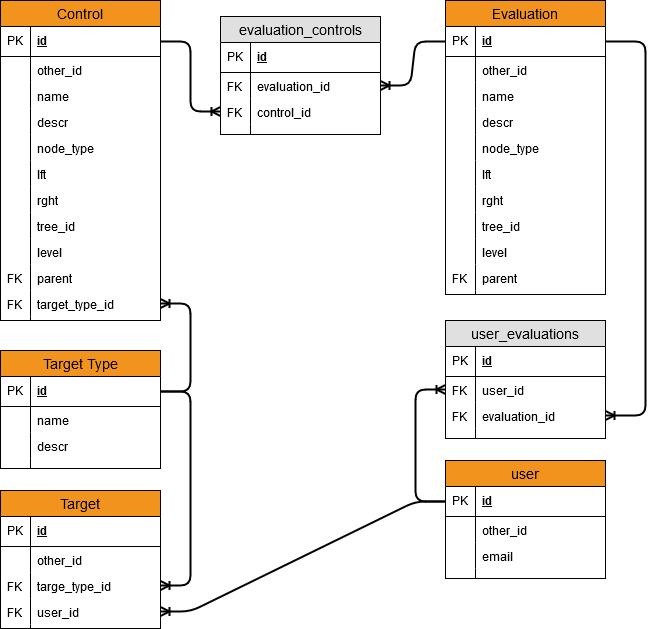
\includegraphics[scale=0.7]{images/MoonCloudRecommendation_ER.png}
	\caption{Struttura del database}
	\label{fig:str_db_project}
\end{figure}

\newpage

% VIEW A SCOPO DIDATTICO
Successivamente per poter testare che la tassonomia creata per le Evalution e i Controlli fosse corretta e funzionante si è 
implementata un'interfaccia Web a scopo didattico.
Avviando il server, la home page che viene prooposta è mostrata nella Figura \ref{fig:MCRS_homepage}, dalla quale è possibile 
accedere alle pagine specifiche per la navigazione della tassonomia delle Evaluation piuttosto che dei Controlli; inoltre 
tramite la barra di navigazione è possibile tornare a questa home page o accedere alla admin page generata da Django, e
succesivamente personalizzata, per poter manipolare la base di dati.\\

\begin{figure}[ht!]
	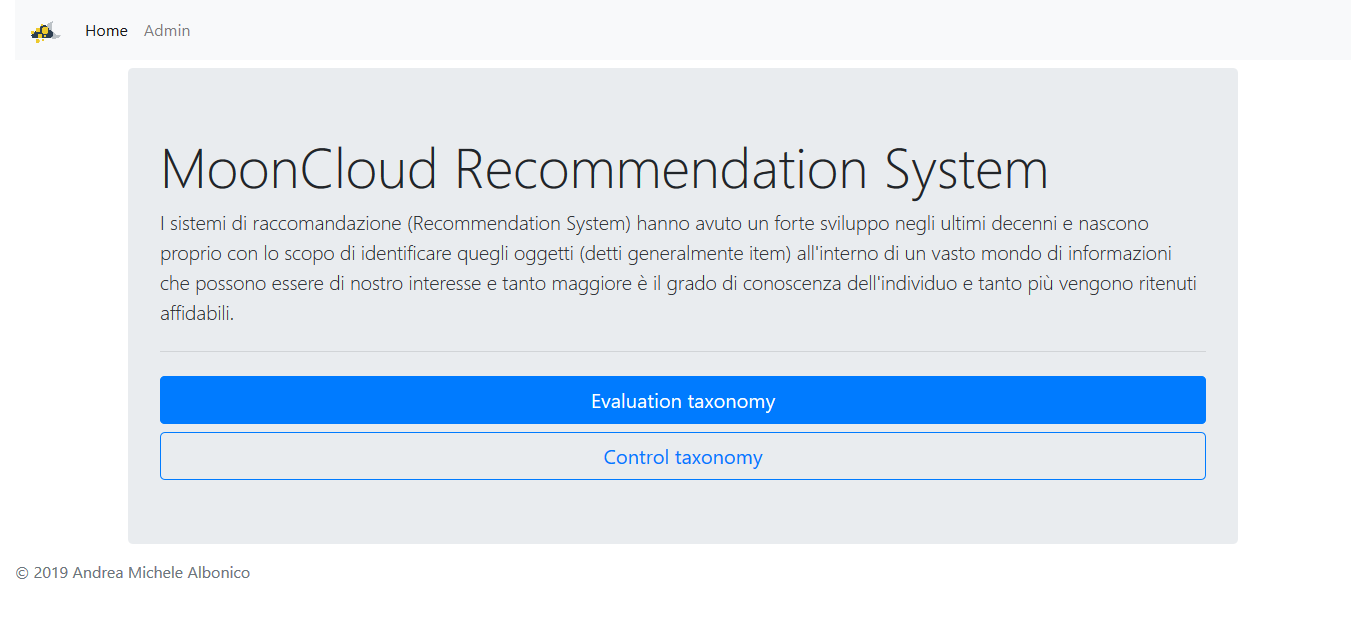
\includegraphics[scale=0.3]{images/MCRS_homepage.png}
	\caption{Home page}
	\label{fig:MCRS_homepage}
\end{figure}

\lstset{style=python_code_style}
\label{lst:view_homepage}
\begin{lstlisting}[language=Python, caption={Parte principale del codice delle View della soluzione per gestire l'accesso
	alla home page}]
# Index page where you can choose to navigate the evaluation taxonomy or the control taxonomy
def index(request):
	return render(request, "recommendation_app/index.html")
\end{lstlisting}


Una volta scelta la tassonomia su cui si vuole navigare, è possibile, per ogni singolo nodo, recuperare: i 
discendenti, la famiglia, i fratelli, e gli antenati; ed è anche possibile scaricare un file scritto in linguaggio
DOT e un'immagine in formato png rappresentante la gerarchia dei dati contenuti nella base dati. 
Inoltre è possibile osservare in maniera più approfondita le informazioni rilevanti sulla tassonomia contenute nelle tabelle
del database.\\

\begin{figure}
	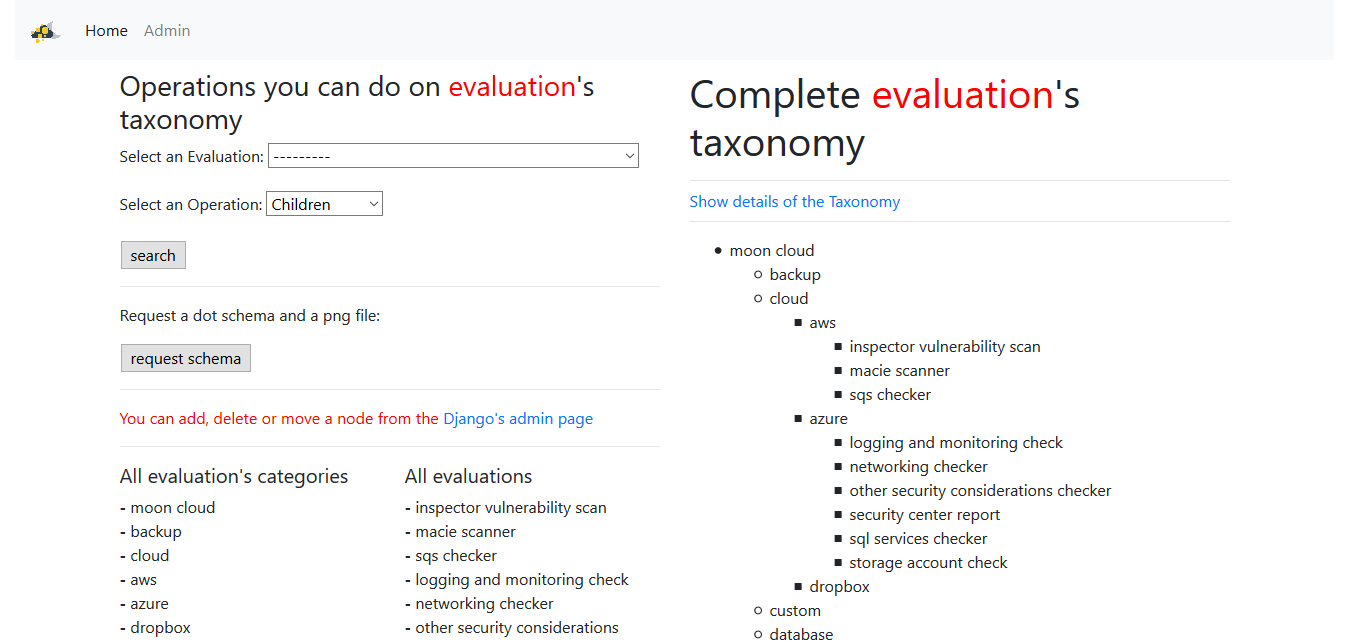
\includegraphics[scale=0.3]{images/MCRS_taxindex.png}
	\caption{Home page per la navigazione della tassonomia}
	\label{fig:MCRS_taxindex}
\end{figure}

\begin{figure}
	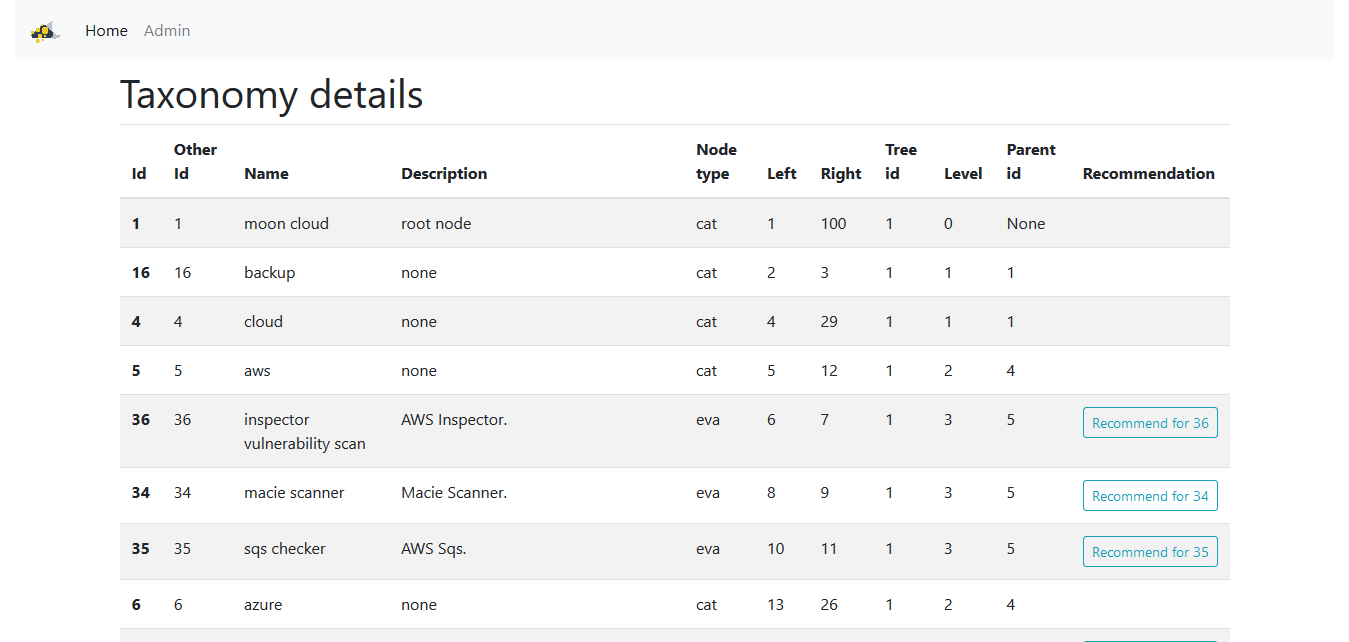
\includegraphics[scale=0.3]{images/MCRS_taxdetails.png}
	\caption{Dettagli della tassonomia sottoforma di tabella come nella base di dati}
	\label{fig:MCRS_taxdetails}
\end{figure}

\begin{figure}
	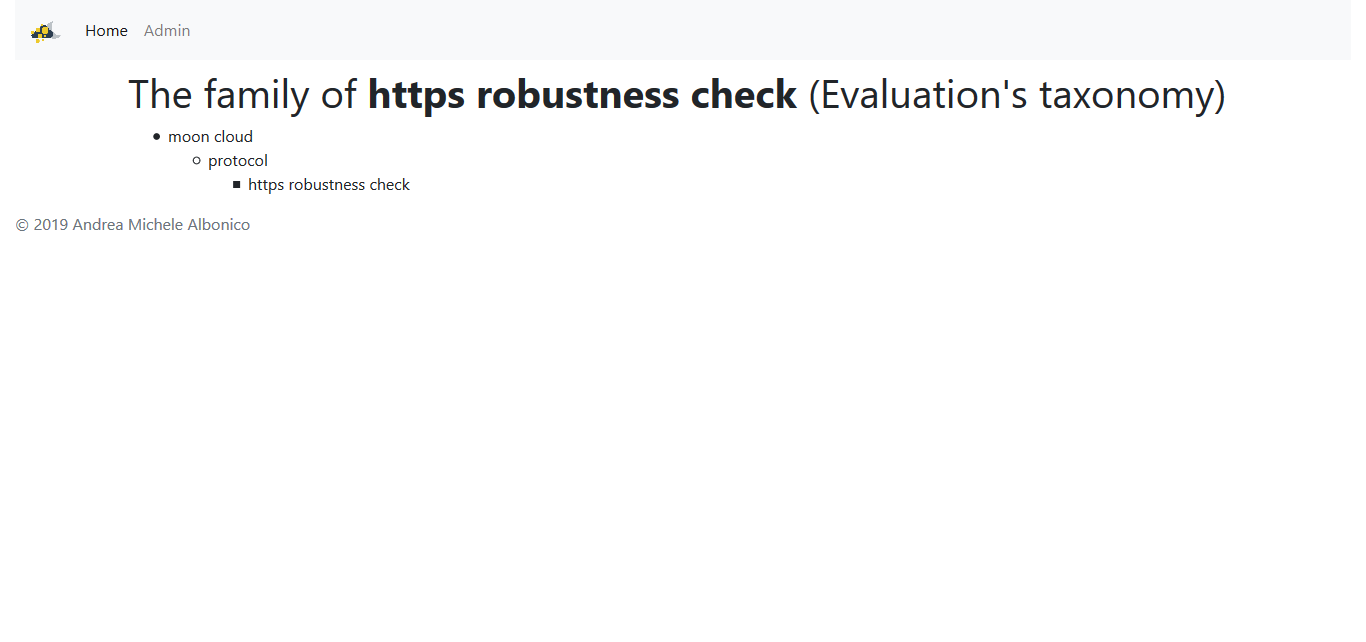
\includegraphics[scale=0.3]{images/MCRS_taxnodedetails.png}
	\caption{Risultato dell'operazione selezionata sul nodo in questione}
	\label{fig:MCRS_taxnodedetails}
\end{figure}

\newpage

Qui di seguito \ref{lst:view} è possibile trovare il codice scritto all'interno delle View per poter eseguire tutte le 
operazioni descritte sopra.

\lstset{style=python_code_style}
\label{lst:view}
\begin{lstlisting}[language=Python, caption={Parti principali del codice delle View della soluzione per gestire la navigazione 
	delle tassonomie, quella delle Evaluation e quella dei Controlli}]

# The home page shows all taxonomy and a form to make operations on it
def tax_index(request, parameter):
	# If this is a POST request we need to process the form data
	if request.method == 'POST':
		# Create a form instance and populate it with data from depending on the parameter
		if (parameter == "evaluation"):
			form = EvaluationOperationForm(request.POST)
		else:
			form = ControlEvaluationForm(request.POST)
		# Check whether it's valid:
		if form.is_valid():
			# Process the data in form.cleaned_data as required
			nodename_form = form.cleaned_data['nodeName']
			taxonomy_operation_form = form.cleaned_data['actionTax']
			# Redirect to a new URL (page that show a part of the taxonomy, depending on the action user has chosen):
			return redirect(
				reverse('rec:tax_index', args=[parameter]) + str(nodename_form) + '_' + taxonomy_operation_form)
	# If id's a GET method we'll create a blank form
	else:
		if (parameter == "evaluation"):
			form = EvaluationOperationForm()
		else:
			form = ControlEvaluationForm()

	# Depending on the parameter, I'm getting all the categories of Evaluations or Controls taxonomy and save it in a
	# list called "categories_list"
	if (parameter == "evaluation"):
		q_categories = Evaluation.objects.filter(node_type='cat')
	else:
		q_categories = Control.objects.filter(node_type='cat')
	categories_list = []
	for node in q_categories:
		categories_list.append(node.name)

	# Depending on the parameter, I'm getting all the categories of Evaluations or Controls node in the taxonomy
	# and save it in a list called "node_list"
	if (parameter == "evaluation"):
		q_nodes = Evaluation.objects.filter(node_type='eva')
	else:
		q_nodes = Control.objects.filter(node_type='con')
	node_list = []
	for node in q_nodes:
		node_list.append(node.name)

	# Depending on the parameter, I'm getting all the Evaluations or Controls taxonomy
	if (parameter == "evaluation"):
		tax = Evaluation.objects.all()
	else:
		tax = Control.objects.all()

	# Passing the complete taxonomy and data to fill the form so you can operate on the taxonomy
	args = {'tax': tax,
			'categories': categories_list,
			'nodes': node_list,
			'form': form,
			'request_path': parameter}

	return render(request, "recommendation_app/tax_index.html", args)


# Show the taxonomy's details page showing an overview of the taxonomy
def tax_details(request, parameter):
	if (parameter == 'evaluation'):
		tax_details_obj = Evaluation.objects.all()
	else:
		tax_details_obj = Control.objects.all()

	return render(request, "recommendation_app/tax_details.html",
				  {'tax_details': tax_details_obj,
				  'parameter': parameter})


# Create the .dot file (based on the Dot language) and the graph showing the taxonomy in .png format
def dot_graph(request, parameter):
	# Create a graph object
	taxonomy_dot_object = Graph(comment='Taxonomy', format='png')
	# Fill the graph with every node in the database (evaluations/controls node and categories nodes), 
	# and create a link with the parent node
	if (parameter == 'evaluation'):
		taxonomy_nodes = Evaluation.objects.all()
	else:
		taxonomy_nodes = Control.objects.all()
	i = 0
	for node in taxonomy_nodes.order_by('level'):
		# This If construct will prevent the adding of an empty node to the root node in the graph
		if (i == 0):
			# Insert the root node
			taxonomy_dot_object.node(str(node.id), label=str(node.name))
		else:
			# Insert the other nodes
			taxonomy_dot_object.node(str(node.id), label=str(node.name))
			taxonomy_dot_object.edge(str(node.parent_id), str(node.id))
		i += 1
	# Specify where I want to save the .png image and the .dot file
	taxonomy_dot_object.render('taxonomy_output/taxonomy.dot')

	# This function is used to zip a directory
	def make_zipdir(path, ziph):
		# Ziph is zipfile handle
		for root, dirs, files in os.walk(path):
			for file in files:
				ziph.write(os.path.join(root, file))

	# Making the zip file
	zip_file = zipfile.ZipFile('taxonomy_output.zip', 'w', compression=zipfile.ZIP_DEFLATED)
	make_zipdir('taxonomy_output/', zip_file)
	zip_file.close()

	# Remove the directory which was zipped and all files inside
	shutil.rmtree("taxonomy_output/")

	return redirect(reverse('rec:index'))


# Method to navigate the taxonomy


# Based on the MPTT's method 'get descendants' that return the descendants of a model instance, in tree order
def show_descendants(request, nodename, parameter):
	if (parameter == 'evaluation'):
		q_result = Evaluation.objects.get(name=nodename).get_descendants(include_self=False)
		# Get the count of descendants of the model instance
		q_result_num = Evaluation.objects.get(name=nodename).get_descendant_count()
	else:
		q_result = Control.objects.get(name=nodename).get_descendants(include_self=False)
		# Get the count of descendants of the model instance
		q_result_num = Control.objects.get(name=nodename).get_descendant_count()

	return render(request, "recommendation_app/tax_node_details.html",
				  {'tax_type': (str(parameter)).capitalize(),
				  'descendants': q_result,
				  'node_exe': nodename,
				  'method': 'descendants',
				  'num_descendants': q_result_num})


# Based on the MPTT's method 'get children' that return the immediate children of a model instance, in tree order
def show_children(request, nodename, parameter):
	if (parameter == 'evaluation'):
		q_result = Evaluation.objects.get(name=nodename).get_children()
	else:
		q_result = Control.objects.get(name=nodename).get_children()

	return render(request, "recommendation_app/tax_node_details.html",
				  {'tax_type': (str(parameter)).capitalize(),
				  'children': q_result,
				  'node_exe': nodename,
				  'method': 'children'})


# Based on the MPTT's method 'get family' that return the ancestors, the model instance itself and the descendants,
# in tree order
def show_family(request, nodename, parameter):
	if (parameter == 'evaluation'):
		q_result = Evaluation.objects.get(name=nodename).get_family()
	else:
		q_result = Control.objects.get(name=nodename).get_family()

	return render(request, "recommendation_app/tax_node_details.html",
				  {'tax_type': (str(parameter)).capitalize(),
				  'family': q_result,
				  'node_exe': nodename,
				  'method': 'family'})


# Based on the MPTT's method 'get siblings' that return siblings of the model instance (root nodes are considered
# to be siblings of other root nodes)
def show_siblings(request, nodename, parameter):
	if (parameter == 'evaluation'):
		q_result = Evaluation.objects.get(name=nodename).get_siblings()
	else:
		q_result = Control.objects.get(name=nodename).get_siblings()

	return render(request, "recommendation_app/tax_node_details.html",
				  {'tax_type': (str(parameter)).capitalize(),
				  'siblings': q_result,
				  'node_exe': nodename,
				  'method': 'siblings'})
\end{lstlisting}


% ASPETTI DI DJANGO CHE HO PERSONALIZZATO, COME LE ADMIN PAGE
Per poter agilmente manipolare la base di dati, Django mette a disposizione la cosidetta Admin Page mostrata in 
Figura \ref{fig:MCRS_adminpage}, che è stata personalizzata per mostrare le tabelle su cui è possibile
effetuare modifiche, e per ognuna vengono mostrate le informazioni più rilevanti, come mostrato dalla 
Figura \ref{fig:MCRS_adminpage_evaluationEX} nel caso della tabella Evaluation, e dalla quale è possibile 
effetuare ricerche, eliminare direttamente i dati contenuti nel database e aggiungere
nuovi dati, come mostrato in Figura \ref{fig:MCRS_adminpage_evaluationEX_add}.\\

\begin{figure}
	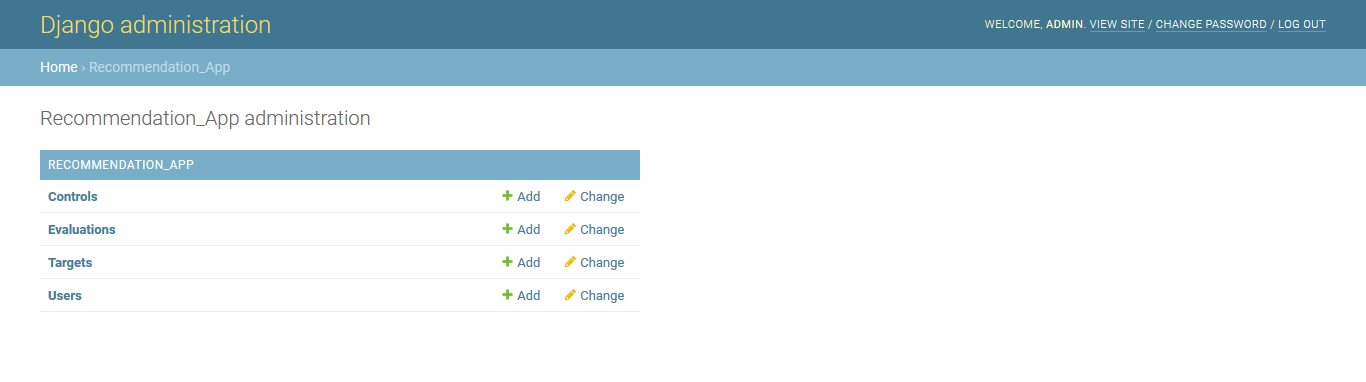
\includegraphics[scale=0.3]{images/MCRS_adminpage.png}
	\caption{Admin page}
	\label{fig:MCRS_adminpage}
\end{figure}

\begin{figure}
	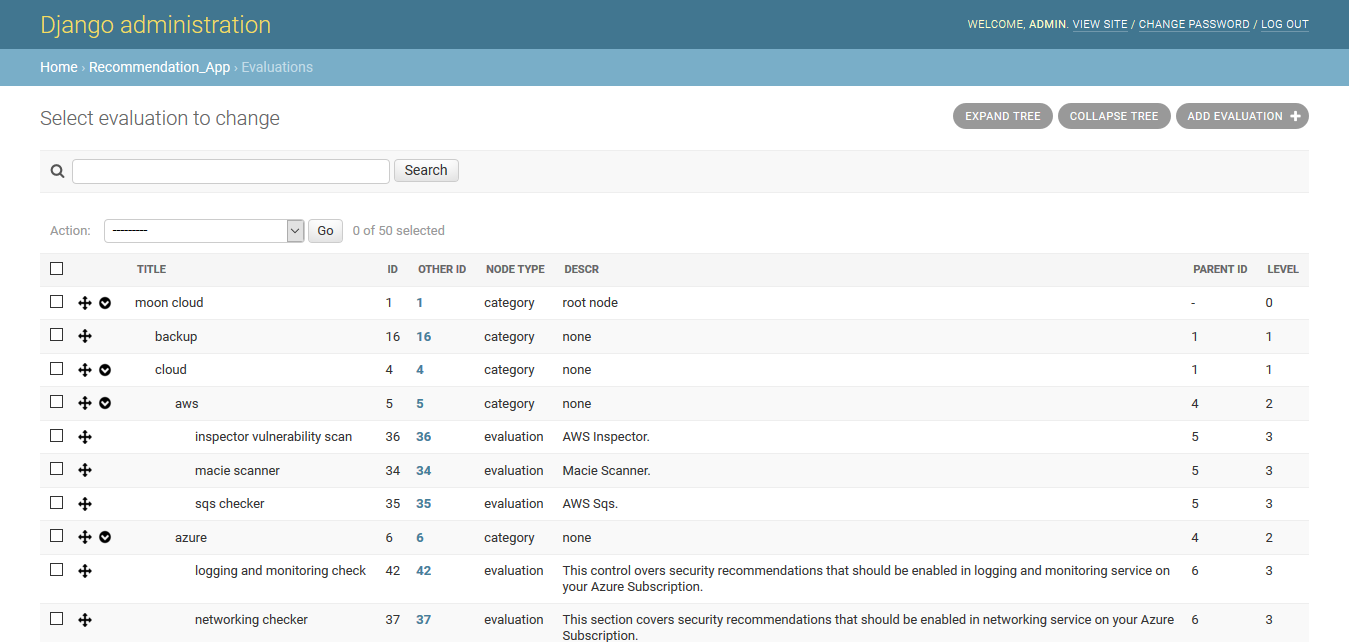
\includegraphics[scale=0.3]{images/MCRS_adminpage_evaluationEX.png}
	\caption{Esempio di Admin page per le Evaluation}
	\label{fig:MCRS_adminpage_evaluationEX}
\end{figure}

\begin{figure}
	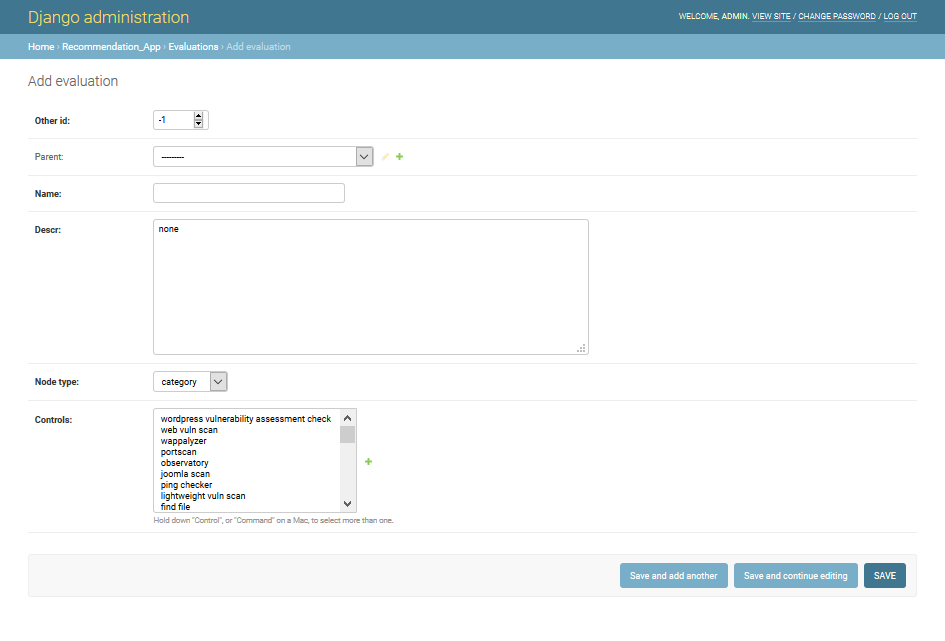
\includegraphics[scale=0.55]{images/MCRS_adminpage_evaluationEX_add.png}
	\caption{Esempio di Admin page per il caso in cui si vuole aggiungere una nuova Evaluation}
	\label{fig:MCRS_adminpage_evaluationEX_add}
\end{figure}

% VIEW PER LE RACCOMANDAZIONI

% VIEW PER MANTERE LA CONSISTENZA COL MIO DATABASE

% IMPLEMENTAZIONE CON DOCKER

